\documentclass[
  language=kz,   % ru (default) | kz | both
  year=2026,     % default: current year
  grade=11,      % default: 11
  tour=theory,   % theory (default) | experiment
  type=solutions  % preview (tbd) | problems (default) | solutions | marking
]{olympiad}

\usepackage{olympiad-layout}
\usepackage{olympiad-units-kz}
\usepackage{olympiad-marking}

% ---- from olympiad.cls itself (Parts 7-12) ----
\SetOlympString{problem}{Есеп}
\SetOlympString{solutions}{Шешiмдер}
\SetOlympString{hints}{Подсказки}
\SetOlympString{consts}{Физические константы}
\SetOlympString{solutionsheader}
{%
    \ifOlympTheory ТЕОРИЯЛЫҚ ТУРДЫҢ ШЕШIМI\fi%
    \ifOlympExperiment ЭКСПЕРИМЕНТАЛДЫҚ ТУРДЫҢ ШЕШIМI\fi%
}
\SetOlympString{figlabel}%
{%
    \ifOlympProblems%
    \theproblemnum\printcounter{subproblemnum}.\thefigcounter-сурет.%
    \fi%
    \ifOlympSolutions%
    \thesolnum\printcounter{subsolnum}.\thefigcounter-сурет.%
    \fi%
    \ifOlympMarking%
    \thesolnum\printcounter{subsolnum}.\thefigcounter-сурет.%
    \fi
}
% #1=caption's prefix (unused), #2=figcounter value; optional, guarded by \@ifundefined in the cls

% ---- from olympiad-layout.sty (Part 7 — used on every normal page) ----
\SetOlympString{name}{Республикалық олимпиада}                 % competitions.yaml: name.short.ru
\SetOlympString{tourname}
{%
    \ifOlympTheory Теориялық тур\fi%
    \ifOlympExperiment Эксперименталдық тур\fi%
}
\SetOlympString{page_abbrev}{б.}
\SetOlympString{duration}
{
    \ifOlympTheory Турдың уақыты --- 5 сағат\fi%
    \ifOlympExperiment Турдың уақыты — 3 сағат\fi%
}
\SetOlympString{organizer}{<<ДАРЫН>> РЕСПУБЛИКАЛЫҚ ҒЫЛЫМИ-ПРАКТИКАЛЫҚ ОРТАЛЫҒЫ} % competitions.yaml: organizer.uppercase.ru
\SetOlympString{city}{Астана}
\SetOlympString{firstpagesubtitle}{\OlympString{name}. \OlympString{tourname}, \OlympGrade{} сынып. \OlympString{city} қ-сы, \OlympYear{}}

\SetOlympString{marking_content}{\textbf{Мазмұны}}
\SetOlympString{marking_total}{\textbf{Барлығы}}
\SetOlympString{eq_formula}{Формула}
\SetOlympString{eq_numerical}{Сандық мән}
\SetOlympString{marking_points}{\textbf{Ұпайлар}}
\SetOlympString{marking_scheme}{Марк-схема}
\SetOlympString{grade_text}{сынып}
\SetOlympString{marking_jury}{Тексеруші}
\SetOlympString{marking_cipher}{Шифр}

\SetOlympString{points_short}{ұпай}
\SetOlympString{points_long}{ұпай}

% ---- from title_ru.tex ----
\SetOlympString{name_full}{Физика пәнi бойынша \OlympString{name}} % competitions.yaml: name.full.ru
\SetOlympString{stage}{Қорытынды кезең}                              % competitions.yaml: name.stage.ru
\SetOlympString{eventdates}{\OlympYear{} жылдың 20-25 наурызы, \OlympString{city}~қ-сы}           % manifest.yaml: dates.opening-ceremony (20) .. dates.closing-ceremony (25), month 3, year 2026

% ---- from templates/instructions_students/theory_ru.tex ----
\SetOlympString{touronedate}{21 наурыз, \OlympYear{} жыл}   % manifest.yaml: dates.first-tour (day 21, month 3), year from dates.year
\SetOlympString{tourtwodate}{22 наурыз, \OlympYear{} жыл}
\SetOlympString{problemcount}{3}                   % manifest.yaml: grades.11.theory has 3 entries

\begin{document}
\solutionsheader

\solution{Қоспа}{10.0}

\subsolution{Үйкеліс арқылы дәнекерлеу}{3.5}

Алдымен үйкелістен бөлінетін қуатты анықтайық. $dS$ аудан бірлігіндегі жылулық шығындардың қуаты:

\begin{eq}[points=0.3]
dP = \mu\cdot p dS\cdot \omega r,
\end{eq}

\criterion[type=remark]{Балл $\omega r\Leftrightarrow v$ немесе $dS\Leftrightarrow2\pi rdr\Leftrightarrow rd\varphi dr$ немесе $pdS\Leftrightarrow dN$ жазбалары үшін де қойылады. $P=\mu N v$ немесе басқа \textbf{инфинитезималды емес} жазбалар үшін балл қойылмайды.}

мұндағы $r<R$ --- айнымалы радиус. $dS = 2\pi r dr$ екенін ескеріп, интегралдау арқылы келесіні аламыз:

\begin{eq}[points=0.5]
P = \frac23 \mu p\omega \pi R^3.
\end{eq}

\criterion[type=penalty, points=-0.3]{$2/3$ коэффициентінің орнына $1$ немесе $1/2$ жазылған. Егер \eqref{2} үшін \textbf{нөлдік емес} балл қойылса, онда \eqref{2}-дегі қателік \eqref{6}, \eqref{7} және \eqref{10}-да ескерілуі тиіс.}

Бөлінген жылу екі цилиндрдің осьтері бойымен таралады. Әрі қарай есеп температураның ось бойындағы $x$ координатасына тәуелді $T(x)$ таралуын талдауға және дәнекерлеу центрінде $T=T^*$ шартын қоюға ұласады. $T(-x)=T(x)$ екені анық болғандықтан, қуаттың $x>0$ бағытына кететін жартысын $P/2$ қарастырайық. Бұл есепте жылу тасымалданудың екі механизмі бар: Фурье жылу өткізгіштігі

\begin{eq}
[
    points=0.3,
    tail={. Минус таңбасы міндетті емес, бірақ бұл \eqref{5}-тегі минус таңбасының болуына әсер етеді.}
]
j = -\kappa \pi R^2\frac{dT}{dx},
\end{eq}
бұл $S=\pi R^2$ ауданы арқылы өтетін $j$ жылу ағынын көрсетеді, және ауаға жылу беру (Ньютон--Рихман заңы):

\begin{eq}[points=0.3]
dq = \alpha\cdot 2\pi R dx\cdot(T-T_0).
\end{eq}
Жылу энергиясының үзіліссіздік теңдеуі бойынша $x\ne0$ болғанда, қалыңдығы $dx$ диск үшін,

\begin{eq}
[
    points=0.3,
    tail={. Егер бұл \eqref{3} пен осы теңдеу арасындағы минус таңбаларының сәйкессіздігіне әкелсе, минус таңбасының болмауы \textbf{қабылданбайды}.}
]
j(x+dx)-j(x)=dj=-dq.
\end{eq}

\begin{figure}[!ht]
\centering
\resizebox{0.25\linewidth}{!}{%
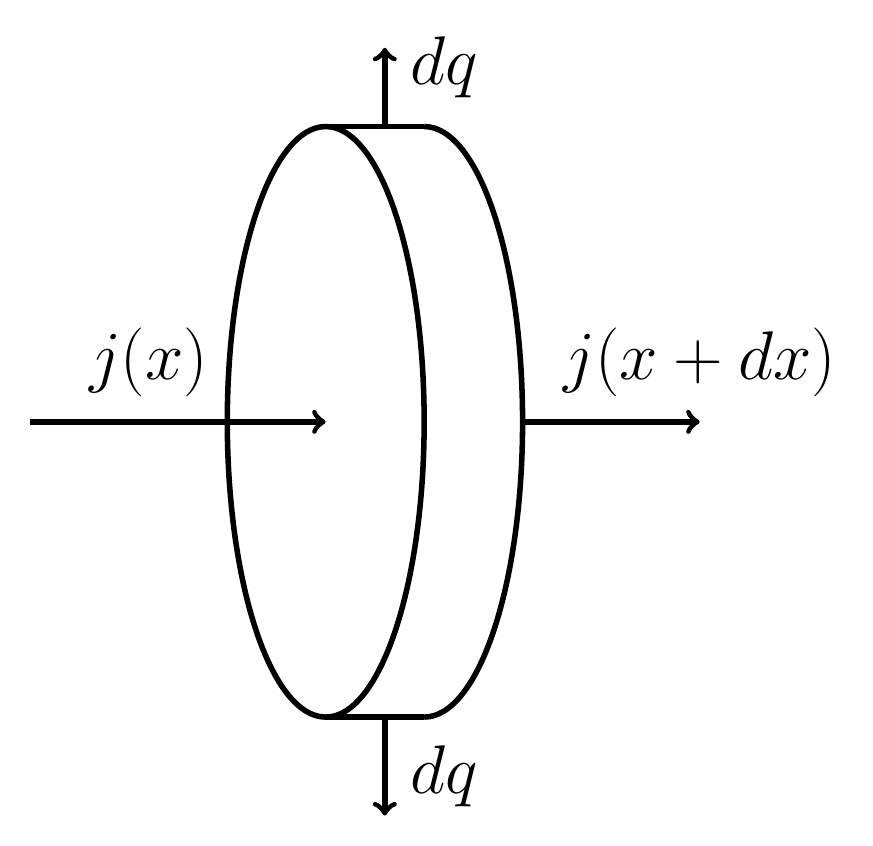
\begin{tikzpicture}[line width=2pt, font=\Huge]
    \draw (13.75, 13.75) ellipse (1.25 and 3.75);
    \draw (15, 17.5) arc (90:-90:1.25 and 3.75);
    \draw (13.75, 17.5) -- (15, 17.5);
    \draw (13.75, 10.0) -- (15, 10.0);
    \draw [->] (10,13.75) -- (13.75,13.75);
    \draw [->] (16.25,13.75) -- (18.5,13.75);
    \node at (11.5,14.5) {$j(x)$};
    \node at (18.5,14.5) {$j(x+dx)$};
    \draw [->] (14.5,17.5) -- (14.5,18.5);
    \draw [->] (14.5,10) -- (14.5,8.75);
    \node at (15.25,18.25) {$dq$};
    \node at (15.25,9.25) {$dq$};
\end{tikzpicture}
}%
\end{figure}

\eqref{3}--\eqref{4} өрнектерін \eqref{5}-ке қоя отырып, келесі түрдегі теңдеуді аламыз:

\begin{eq}[points=0.2]
\frac{d^2T}{dx^2} = \frac{2\alpha}{\kappa R}(T-T_0).
\end{eq}

Бұл --- бұрыштық жиіліктің квадраты теріс болатын ``тербеліс теңдеуі''. Математикалық кеңесті пайдаланып және

\begin{eq}[points=0.2]
\lambda=\sqrt\frac{2\alpha}{\kappa R},
\end{eq}

екенін ескерсек, $x=0$ нүктесіне қатысты симметрияны есепке алғанда, жалпы шешім келесі түрде болуы керек:

\begin{eq}[points=0.4]
T(x)=T_0+A\exp\ab(-\lambda|x|)
\end{eq}

\criterion[type=remark]{Модуль міндетті емес. Егер $T_0$ орнына кез келген \textbf{нөлдік емес} тұрақты тұрса, қабылданады. Басқа жағдайларда балл қойылмайды.}

мұндағы $A$ --- анықталуы тиіс қандай да бір тұрақты. Мұнда теріс $\lambda$ ескерілмейді, өйткені олай болмаған жағдайда оң экспонента шексіздікке кетер еді. Жалпы алғанда, қатысушыдан $x>0$ және $x<0$ жағдайларының екеуін де талдау талап етілмейді, өйткені тек шектік шартты дұрыс табу маңызды. Бізде:

\begin{eq}[points=0.3]
j(0)=\frac P2.
\end{eq}

(Дәлірек айтсақ, $j(0^+)=+P/2$ және $j(0^-)=-P/2$). $T(0)=T^*$ шартын ескере отырып шешсек,

$$
\frac P2 = \kappa \pi R^2 \cdot \ab(\sqrt{\frac{2\alpha}{\kappa R}}\cdot A)\implies  A = \frac{P}{2\pi R\sqrt{2\kappa\alpha R}} = T^* - T_0,
$$

\begin{eq}[points=0.5, numpoints=0.2]
\omega = \frac3{\mu pR}\sqrt\frac{2\kappa\alpha }R\cdot(T^*-T_0)=\qty{51.0}{\radian\per\s}.
\end{eq}

\criterion[type=remark]{Сандық есептеулерде қателіктің көшірілуі (error propagation) жоқ.}

Бұл минутына 500 айналымнан сәл ғана кем. Реалды диапазон минутына 400-ден 1500 айналымға дейінгі аралықты құрайды. Әрине, үйкеліс арқылы дәнекерлеудің нақтырақ механизмдері квазистационарлы бола алмайды, бірақ бұл модель негізгі механизмдерді ескеру арқылы реалды диапазондағы нәтижені жақсы береді.

\input{respa2026_11_1akz_sol_marking_kz.tex}
\input{respa2026_11_1bkz_sol.tex}
\input{respa2026_11_1bkz_sol_marking_kz.tex}
\input{respa2026_11_1ckz_sol.tex}
\input{respa2026_11_1ckz_sol_marking_kz.tex}
\input{respa2026_11_2kz_sol.tex}
\input{respa2026_11_2kz_sol_marking_kz.tex}
\input{respa2026_11_3kz_sol.tex}
\input{respa2026_11_3kz_sol_marking_kz.tex}
\end{document}
